\chapter*{Annexe 2 - Modèles SIMULINK}
\addcontentsline{toc}{chapter}{Modèles SIMULINK}
%\setcounter{section}{0}
% **********************************
\label{Annex:SIMULINK_RE}
\lstset{
  language=Matlab,                	  % choose the language of the code
  basicstyle=\ttfamily,
  numbers=left,                   % where to put the line-numbers
  stepnumber=1,                   % the step between two line-numbers.
  numbersep=5pt,                  % how far the line-numbers are from the code
  backgroundcolor=\color{white},  % choose the background color. You must add \usepackage{color}
  commentstyle = \color{darkgreen},
  showspaces=false,               % show spaces adding particular underscores
  showstringspaces=false,         % underline spaces within strings
  showtabs=false,                 % show tabs within strings adding particular underscores
  tabsize=2,                      % sets default tabsize to 2 spaces
  captionpos=b,                   % sets the caption-position to bottom
  breaklines=true,                % sets automatic line breaking
  breakatwhitespace=true,         % sets if automatic breaks should only happen at whitespace
  %caption=exo1.m,                 % show the filename of files included with \lstinputlisting;
  literate={á}{{\'a}}1 {è}{{\`e}}1 {é}{{\'e}}1,
}

\addcontentsline{toc}{section}{Modèle Global}
\section*{Modèle Global}
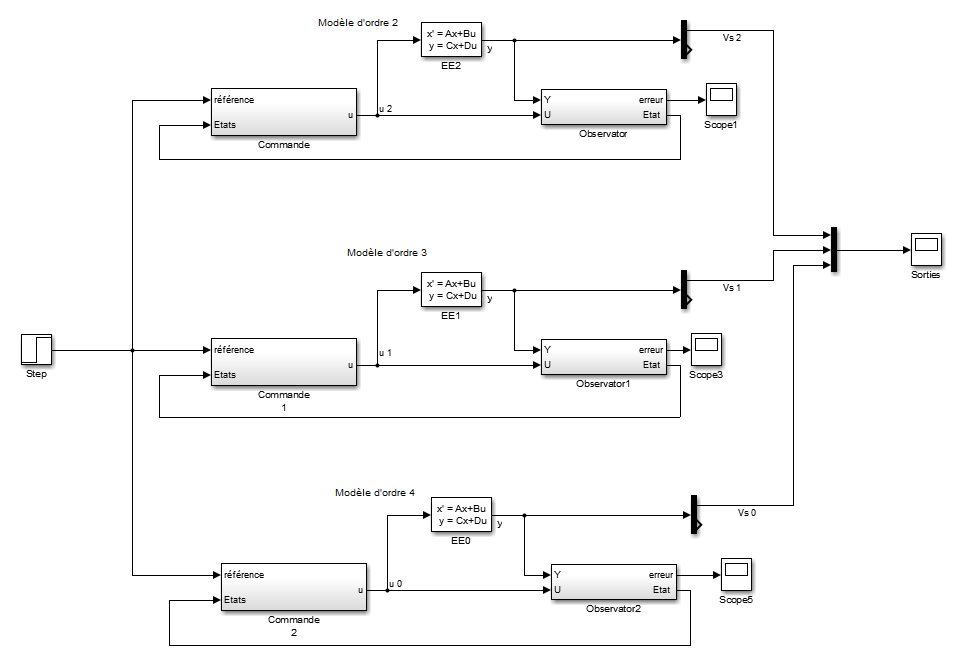
\includegraphics[width = \textwidth]{./annexes/annexe2/simu.PNG}

\addcontentsline{toc}{section}{Sous-système de commande}
\section*{Sous-système de commande}
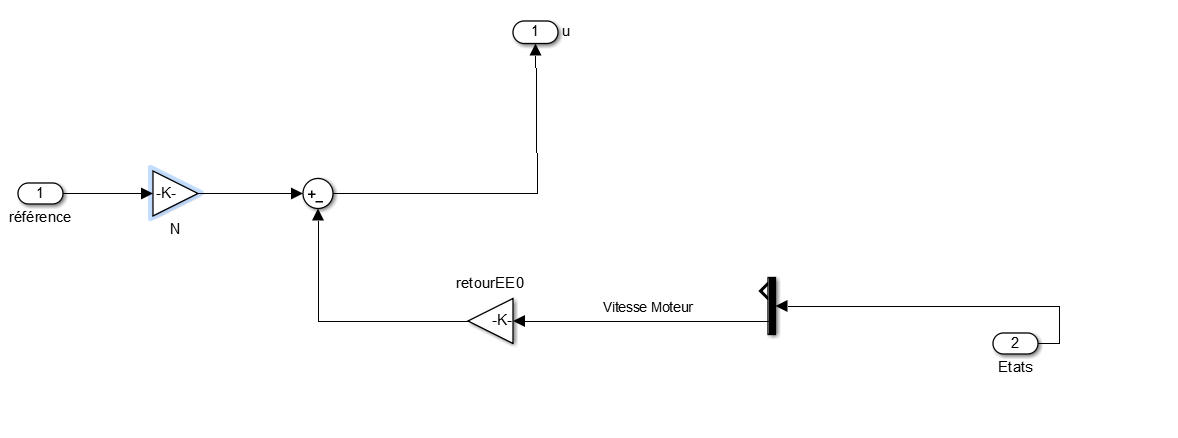
\includegraphics[width = \textwidth]{./annexes/annexe2/Command.PNG}

\addcontentsline{toc}{section}{Sous-système d'observateur}
\section*{Sous-système d'observateur}
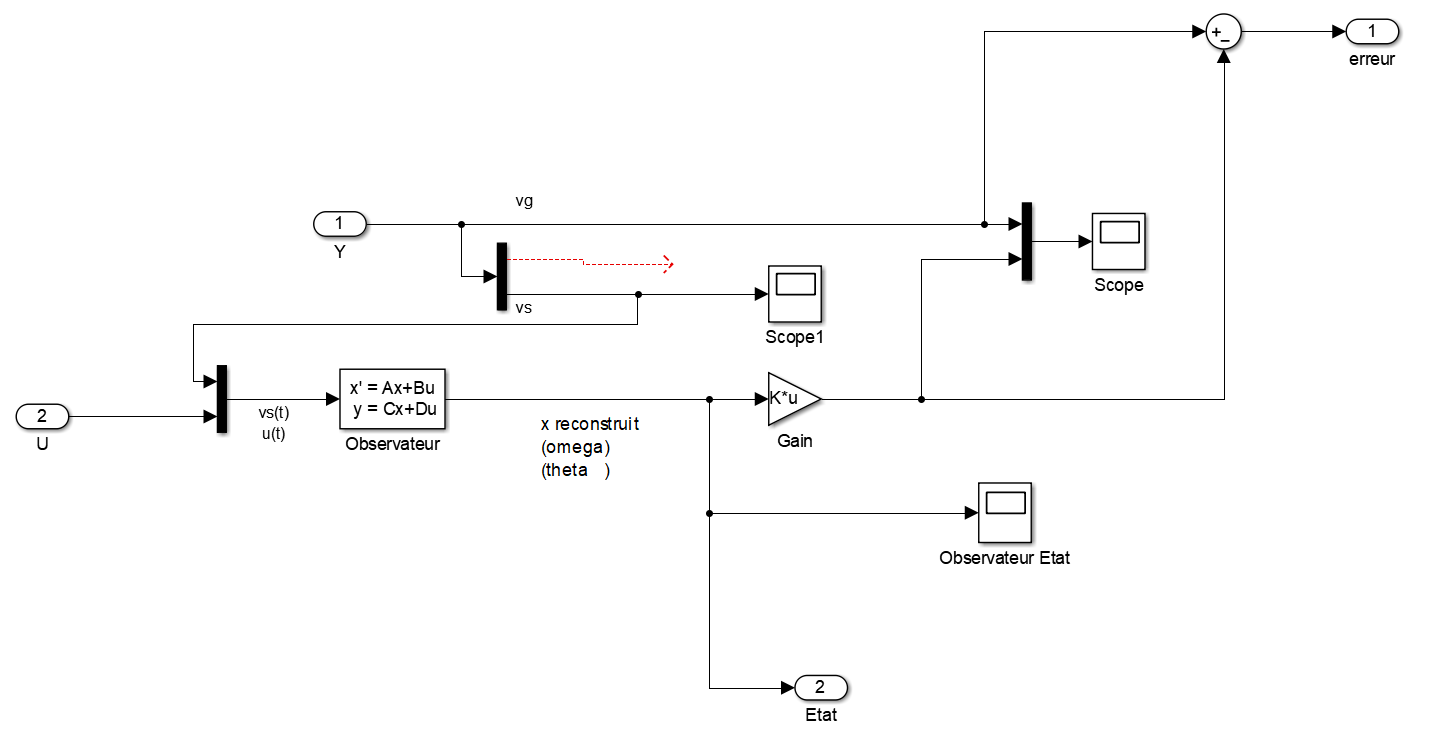
\includegraphics[width = \textwidth]{./annexes/annexe2/Observateur.PNG}